\documentclass{beamer}
\usetheme{Warsaw}

\usepackage[utf8]{inputenc}
\usepackage{fancybox}
\usepackage{multimedia} 
\usepackage{subfig}
\usepackage{amsmath}

\usepackage[all]{xy}
\begin{document}


\title[Computergrafik] % (optional, only for long titles)
{Computergrafik

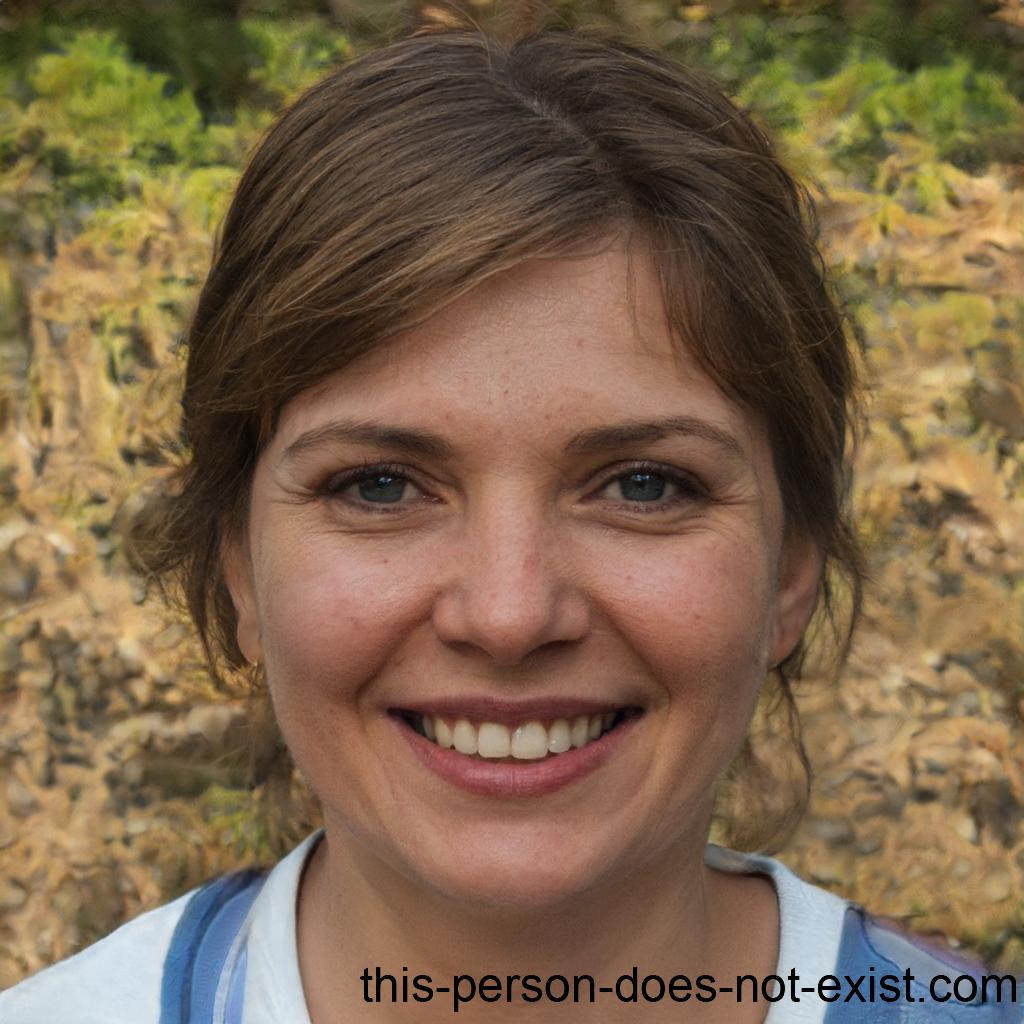
\includegraphics[scale=0.36]{images/person}
}
\subtitle{}
\author[Dr. Johannes Riesterer] % (optional, for multiple authors)
{Dr.  rer. nat. Johannes Riesterer}

\date[KPT 2004] % (optional)
{}

\subject{Computergrafik}


\begin{frame}
    \frametitle{Generative Modelle}
\framesubtitle{}
\begin{block}{Diese Person existiert nicht! https://this-person-does-not-exist.com/de}
    \center
    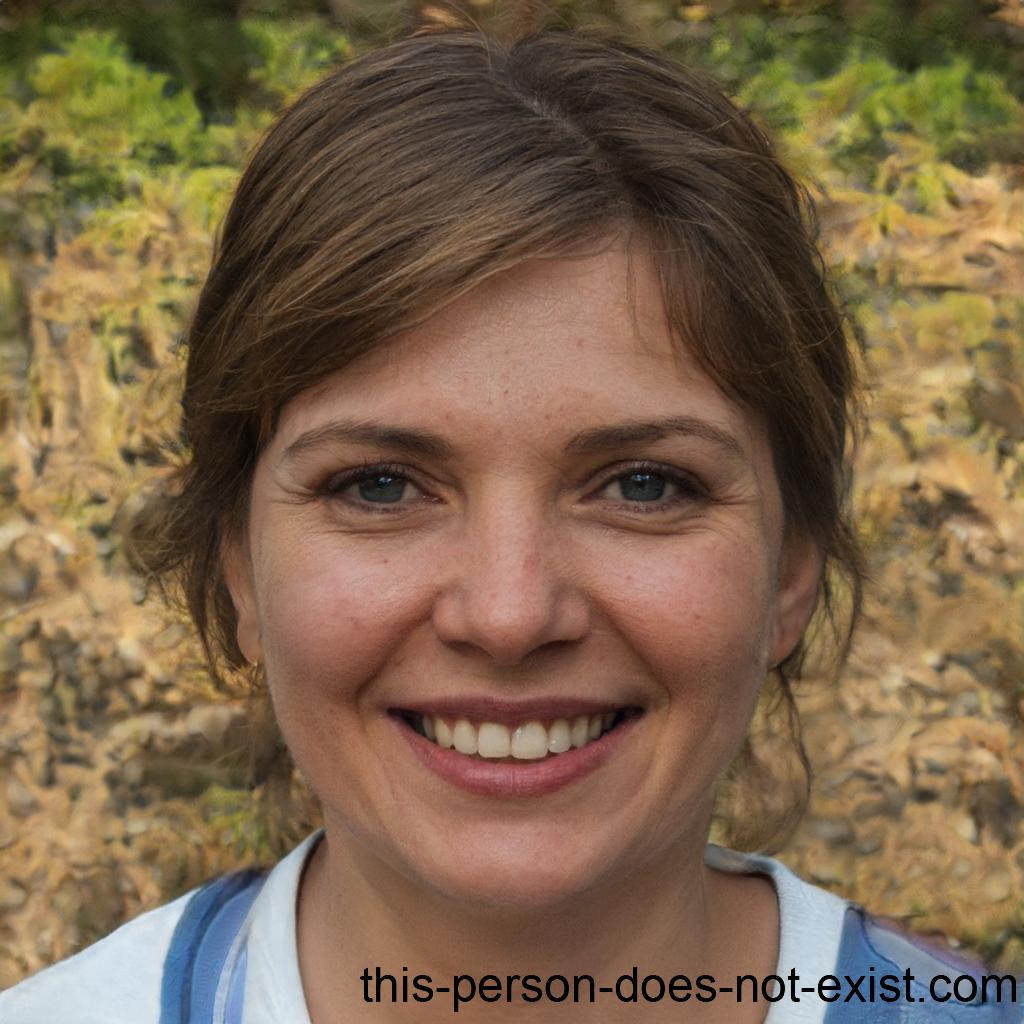
\includegraphics[scale=0.25]{images/person}
\end{block}
\end{frame}


\begin{frame}
    \frametitle{Generative AI}
\framesubtitle{}
\begin{block}{Generative AI (Wiki)}
    Generative künstliche Intelligenz (auch generative KI oder GenAI) bezeichnet künstliche Intelligenz, 
    die in der Lage ist, Texte, Bilder oder andere Medien mithilfe generativer Modelle zu erzeugen. Generative KI-Modelle lernen die Muster und Struktur ihrer Eingabedaten während des Trainings und erzeugen anschließend neue Daten mit ähnlichen Merkmalen.
\end{block}
\begin{block}{Generative AI (ChatGPT (Selbst eine generative AI))}
 
Ein generatives Modell in der künstlichen Intelligenz (KI) ist ein Typ von Modell, 
das darauf abzielt, neue Daten zu erstellen, die ähnlich zu den Trainingsdaten sind, 
mit denen es trainiert wurde. Im Gegensatz zu diskriminativen Modellen, 
die darauf ausgelegt sind, zwischen verschiedenen Klassen oder Kategorien zu unterscheiden, 
versucht ein generatives Modell, 
die Verteilung der Trainingsdaten zu erfassen, um neue Daten zu generieren.
\end{block}
\end{frame}

\begin{frame}
    \frametitle{Generative Modelle}
\framesubtitle{}
\begin{block}{Autoencoder}
    \center
    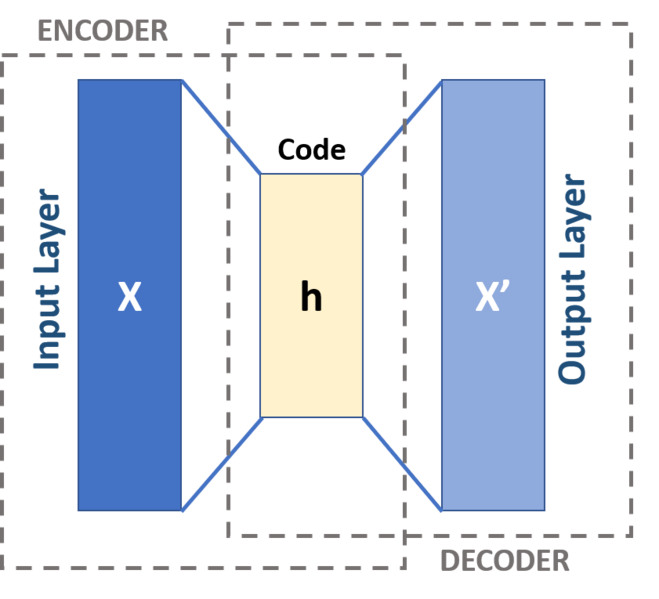
\includegraphics[scale=0.35]{images/autoencoder}
\end{block}
\begin{block}{Autoencoder}
    \center
    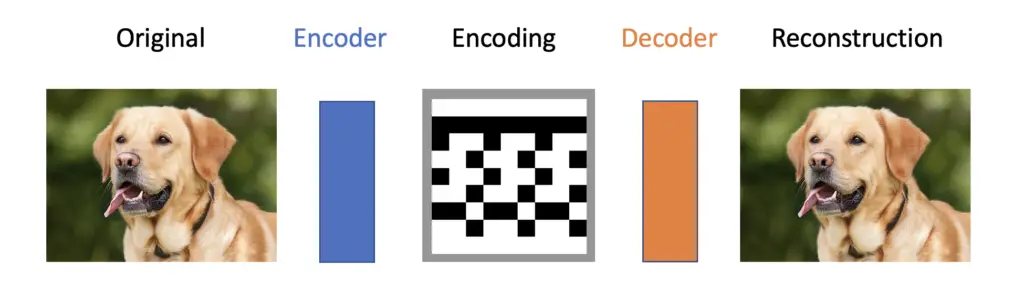
\includegraphics[scale=0.25]{images/autoencoder_train}
\end{block}
\end{frame}



\begin{frame}
    \frametitle{Generative Modelle}
\framesubtitle{}
    \begin{block}{GAN Architektur}
\begin{figure}[H]
    \centering
    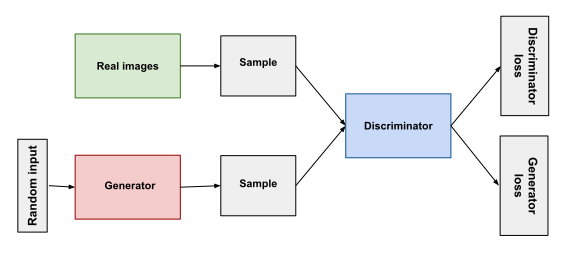
\includegraphics[width=0.6\textwidth]{images/gan_diagram}
\end{figure}
\end{block}
\begin{block}{Generator \& Discriminator}
    \begin{figure}[H]
        \centering
        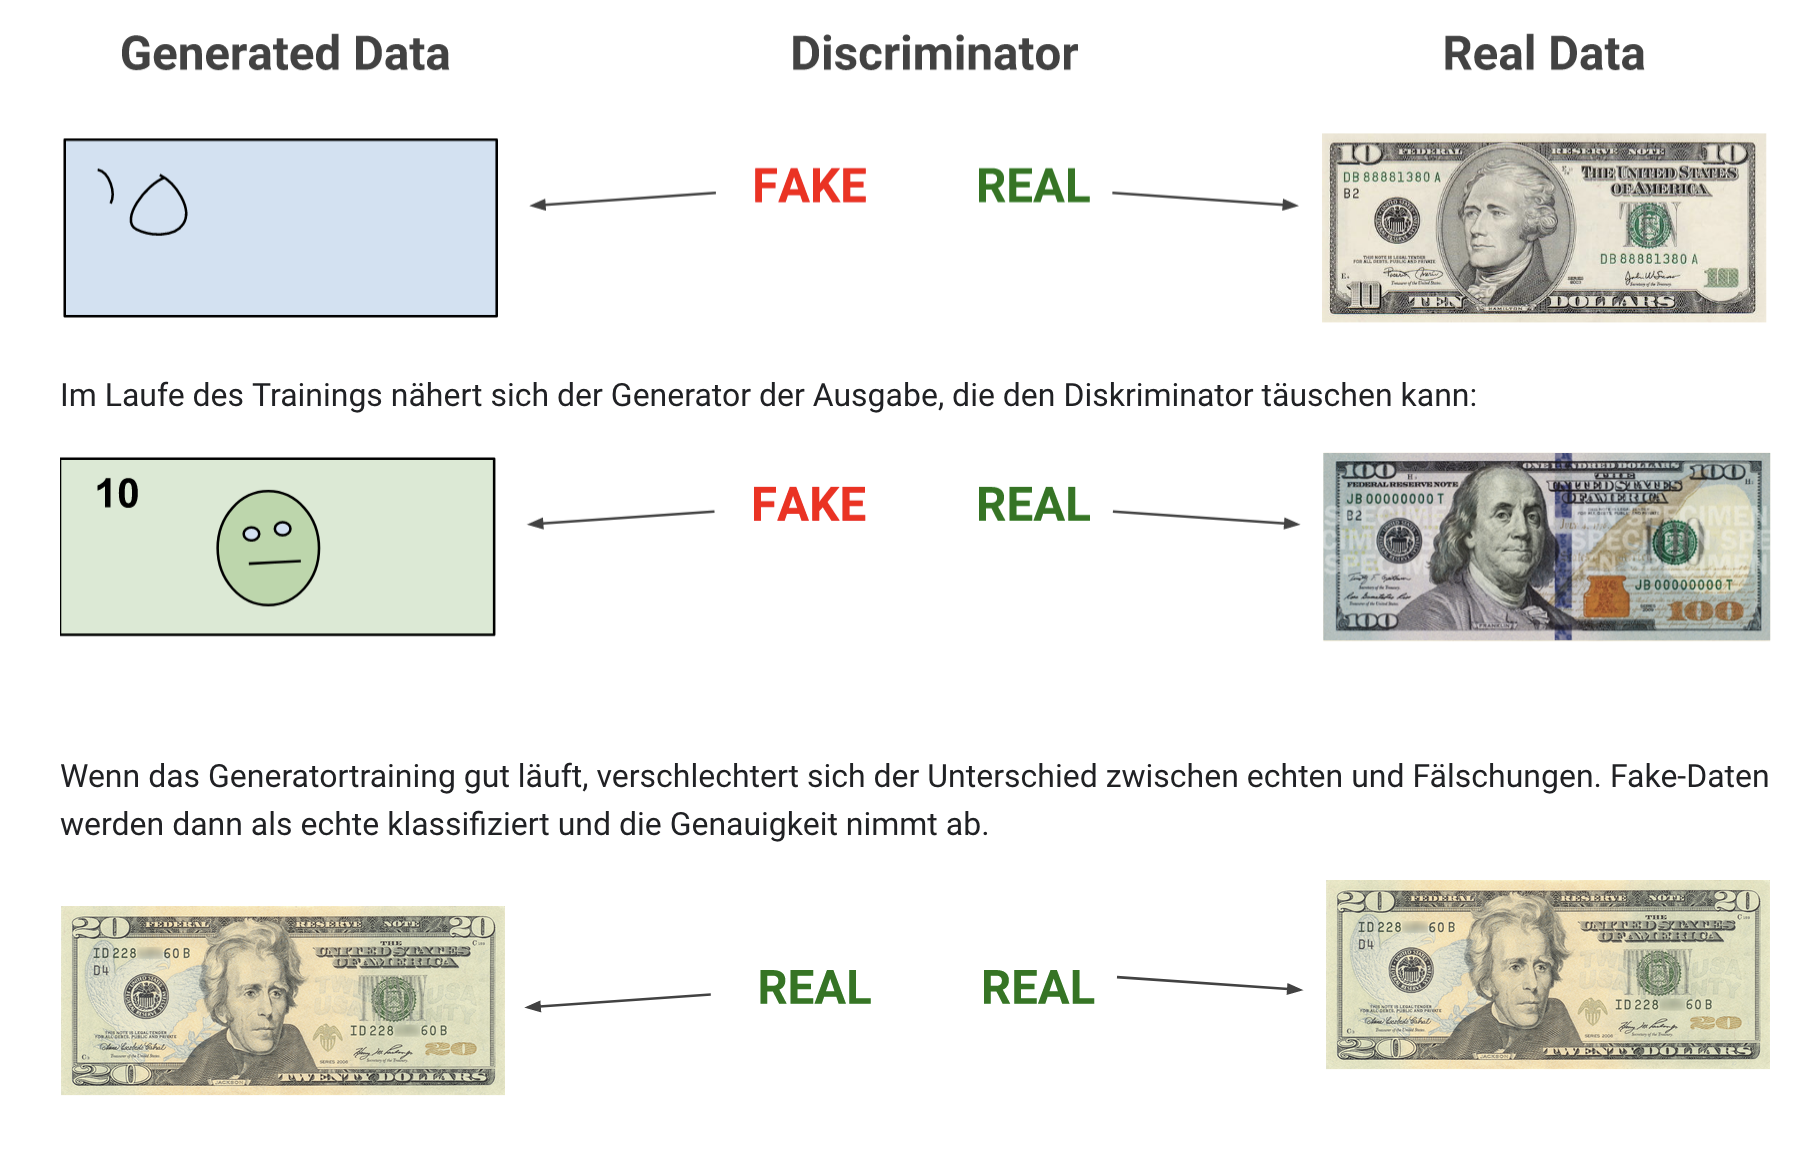
\includegraphics[width=0.45\textwidth]{images/gan_images}
    \end{figure}
    \end{block}
\end{frame}


\begin{frame}
    \frametitle{Generative Modelle}
\framesubtitle{}
    \begin{block}{Training Discriminator}
\begin{figure}[H]
    \centering
    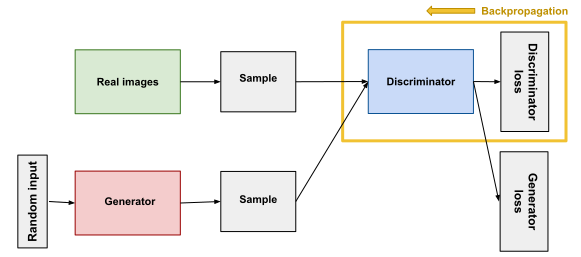
\includegraphics[width=0.55\textwidth]{images/gan_diagram_discriminator}
\end{figure}
\end{block}
\begin{block}{Training Generator}
    \begin{figure}[H]
        \centering
        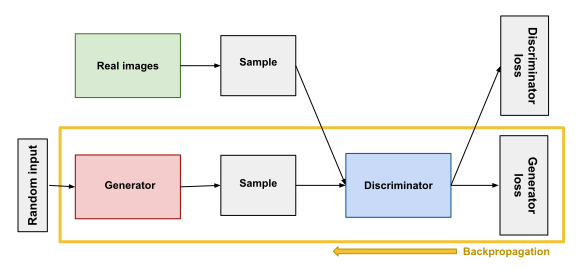
\includegraphics[width=0.55\textwidth]{images/gan_diagram_generator}
    \end{figure}
    \end{block}
\end{frame}


\end{document}
